%
% sample.tex
% $Id: sample.tex,v 1.1 2006/03/18 00:21:36 johnh Exp johnh $
%
% File is renamed to sensys-full.tex to reflect the twists made to use sensys-proc.cls.
% 

% The default of sigplan-proc-varsize is 9pt, indented paragraphs (acm style)
% For Sensys or other 10pt conference, use the 10pt option
%\documentclass{sigplan-proc-varsize}
% options:
%\documentclass[9pt]{sigplan-proc-varsize}
%\documentclass[nocopyrightspace,10pt]{sigplan-proc-varsize-sensys-abstract}

\documentclass[10pt]{sensys-proc}

% % hack to avoid the ugly ACM paragraph definition
% % => can't leave blank line after this
% (remove comment for this hack)
% \renewcommand{\paragraph}[1]{\vskip 6pt\noindent\textbf{#1 }}

\usepackage{graphicx}
\usepackage{balance}
\usepackage{comment}

\numberofauthors{2}

\author{
%
% The command \alignauthor (no curly braces needed) should
% precede each author name, affiliation/snail-mail address and
% e-mail address. Additionally, tag each line of
% affiliation/address with \affaddr, and tag the
%% e-mail address with \email.
% \alignauthor Alice Security \\
%         \affaddr{Department of Computer Science}\\
%         \affaddr{University of Southern California}\\
%        \email{alice@example.edu}
% \alignauthor Bob Privacy \\
%     \affaddr{Networked Embedded Systems Group}\\
%     \affaddr{Swedish Institute of Computer Science}\\
%     \email{bob@example.se}
}

\title{Full Paper for ACM SenSys Proceedings}

\crdata{978-1-4503-1169-4}
\conferenceinfo{SenSys'13,} {November 11--15, 2013, Rome, Italy.}
\CopyrightYear{2013}

\begin{document}

\maketitle

\begin{abstract}
More than 70\% of commercial buildings have giant sensor networks to monitor different aspects of building performance. However, most of these deployed sensor networks have little metadata describing context, which precludes writing analytics applications without familiarity of the particular building’s sensor metadata structure. 

In this paper, we propose a technique which learns how to transform a building’s metadata to a common namespace by using a small number of examples from an expert. Once the transformation rules are learnt for one building, it can be applied across buildings with a similar metadata structure. We illustrate this on a testbed consisting of 60 buildings comprising more than 20,000 sensor points. We also illustrate how this common namespace can help a user write analytics applications that do not require building-specific knowledge, and also scales across different buildings. 
\end{abstract}

% A category with the (minimum) three required fields
% \category{H.4}{Information Systems Applications}{Miscellaneous}
% %A category including the fourth, optional field follows...
% \category{D.2.8}{Software Engineering}{Metrics}[complexity measures, performance measures]

% \terms{Delphi theory}

% \keywords{ACM proceedings, \LaTeX, text tagging}

\section{Introduction}

Buildings are sites of very large sensor deployments, typically containing
up to several thousand sensors reporting physical measurement, continuously.
Moreover, with the recent interest in reducing building energy consumption, it
is important to consider ways to quickly bootstrap a set of building data streams
into an anlytical pipeline to determine where there are opportunities for energy savings,
discovery of broken sensors, and assessing and tracking overall building performance.
However, current `point' naming conventions form a bottleneck in the scalability of
the data integration process.  A `point' refers to a physical location where
a sensor is taking measurements. Each building vendor uses their own naming scheme and
uniques variants of each scheme are implemented from building to building; variations exist
even across buildings that have contracted the same vendor to set up their deployment.
This makes the integration process laborious and fundamentally unscalable.  If we
wish to have a broad impact across the entire building stock, at scale, we need
to explore methods for overcoming this challenge.

Consider a simple analysis whcih has the ability
to identify anomalous readings from a specific kind of sensor.  In order to run the application
the deployer needs to know the name of the sensorand how to attain readings from it.
The stream identification process is manual.  The deployer loads the interface to the 
building management system, tracks down the spatial or system view, clicks through several windows
to locate the location of the point(s) of interest, mouses over the point(s) and records the name,
and then uses that point name to request it from the data-fetch protocol -- typically BACNet or 
LonTalk or another protocol. This process is repeated in \emph{every building} where this 
application runs.  Any application that uses building data requires access to the building
management system and the network carrying the data of interest.

In order to meaningfully deal with disparate building streams in a scalable 
fashion the streams should be \emph{searchable} across various properties, such
as building name, room location, and statistical trends.  Moreover, we
assert that wide searchability is necessary for achieving scalability.  By providing a tool for
searching across building streams, we minimize the deployment time for applications that 
allowing them to be used in \emph{all} buildings, not just a single one.  The aforementioned 
building manamgent system user interface implicitly groups sensors by location in space
or association with a system.  This grouping is also captured in the name of the point used by
the underlying communication protocol.  For example, 'AHU' -- air handling unit -- is typically
embedded in the name of every sensor that is associated with a particular air handling unit.
A similar convention is used for denoting the type of data produced by the point (i.e. all points
that contain 'ART' (area room temperature)  in their name refer to a temperature sensor).
However, these conventions vary slightly across buildings, making it difficult to
simply integrate based on such tags alone.  We need a way to unify and learn the basic
set and structure of the tags in order to unify them.

Also, commonality across certain statistical features can be used to group
different streams.  For example, consider the distribution of temperature reading across
the rooms in the building.  Given a value distribution, it might be easy to pick out values those
that classify as statistical anoamlies.  If you consider the distribution per sensor type, then
finding all statistically anomalous sensor might also identify those that are broken.
This can be determined and indexed a priori, easing the time it takes to identify the 
streams of interest to applications.

In this paper, we propose a technique which learns how to transform a building's metadata 
to a common namespace by using a small number of examples from an expert. Once the transformation 
rules are learnt for one building, it can be applied across buildings with a similar 
metadata structure.  We also show how processes that extract statistical features and generate
descriptive metadata can help unify data streams with respect to much deeper attributes.
We show how our approach makes it easier to write applications across buildings by
demonstrating its use by three different applications: 1) a rogue zone detector, 2)
a broken senor finder and 3) an application that identifies and ranks the most comfortable
rooms. We illustrate these on a testbed consisting of 60 buildings comprising more 
than 20,000 sensor points. We also illustrate how this common namespace can help a user write 
analytics applications that do not require building-specific knowledge and scales across 
different buildings. 

% We observe that every naming scheme looks to capture three point attributes: 
% 1) the location in space, 2) its relation to an subsytem, and 3) the type of 
% measurement it is taking.  

% We want to make the streams searchable.  How do we do that?
% ) We need index the metadata for the streams but the metadata available is not enough
% 2) We need to expand the metadata, but how?
% 3) name expansion --> tag unification
% 4) timeseries feature extraction --> tag unification

% top things to expand upon:  location, type, system
% secondary: statistical features about the data
 

\section{Motivation}

Buildings are notoriously complex from a management perspective.  They consume a large fraction
of the energy produced in the United States and much of is wasted~\cite{epa}.  There has been
much work in the building science community to reduce their energy consumption and make them more
efficieny, but the route to broader impact is typically carried out through regulations guided
by the findings of studies in those communities~\cite{regulation}.
We aim to let solutions reach buildings \emph{directly} by making sense of the data they produce
as quickly and accurately as possible.
In order to achieve this at scale, we must explore ways to deal with the data produced
from sensors within them and to enable braod anaysis across several buildings at a time. Our study
focuses on any building equipped with a network of sensors.  Nearly 
three-quarters of commercial buildings contain a rich sensing fabric, installed as part
of the building management system~\cite{study}.  
It is the data from these system and variants of it, that
we wish to unify and make sense of in a more systematic and automated fashion.

Fortunately, we have access to a large corpus of data from buildings on our campus.
We examine the data from 56 buildings containing over 22,600 sense points. These buildings 
represent a vast range in age, size, and density of deployment.  It also represents deployments
that were set up by more than one vendor.  As expected, newer buildings have many more sense 
points than older ones -- although some old buildings that have been retrofitted have over 1000  
points within them. The maximum number of points in a 
single building is 6169 and the minimum is 27.   The built years spans over 100 years -- from 
1905 to 2007. The size range spans over an order of magnitude 
in square footage from about 30,000 square feet to over 360,000 square feet.  The access this
this kind of breadth of system and building types makes our study unique.

\begin{figure*}[h]
\centering
	\begin{subfigure}{0.5\textwidth}
                \centering
		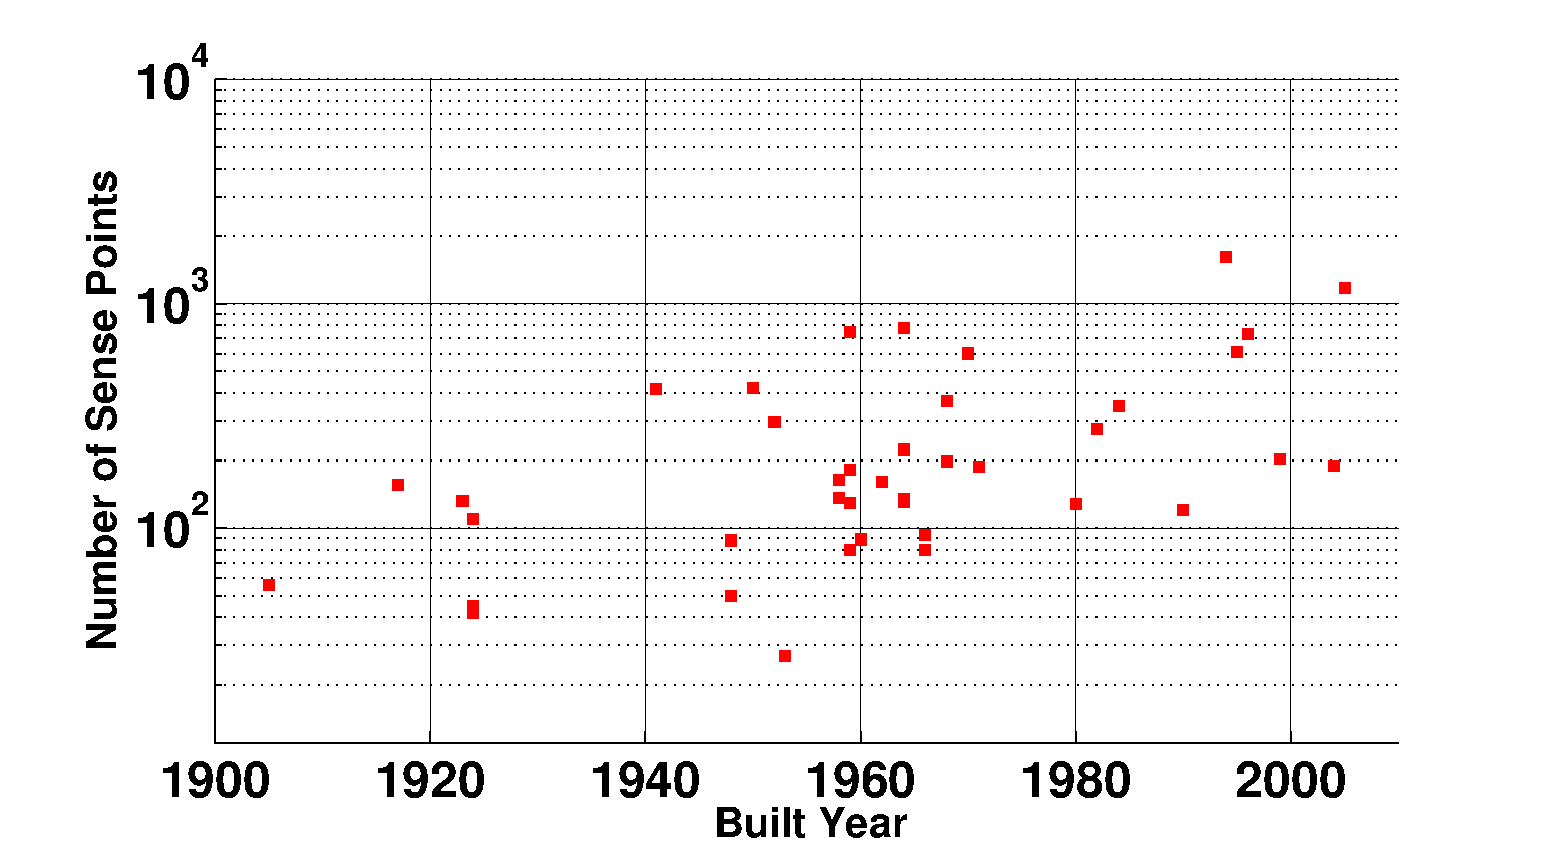
\includegraphics[width=\textwidth]{./figs/pts_vs_yearbuilt.eps}
                \caption{Number of Points vs Year Built}
	\end{subfigure}
	\begin{subfigure}{0.5\textwidth}
                \centering
		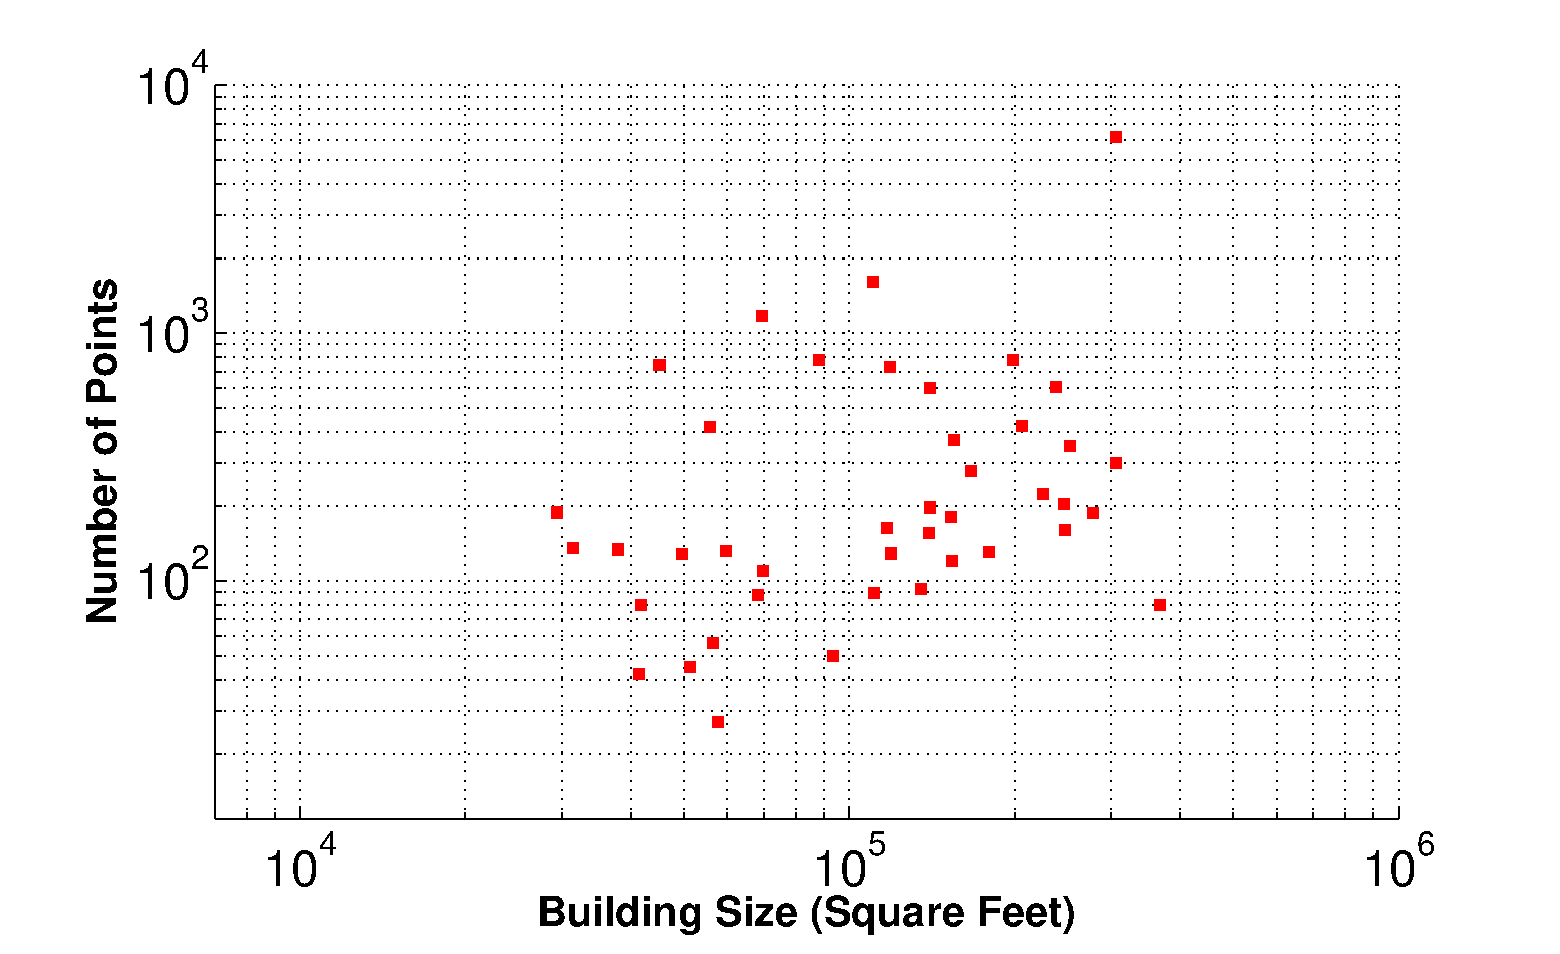
\includegraphics[width=\textwidth]{./figs/pts_vs_buildsz.eps}
                \caption{Number of Points vs Building Size}
	\end{subfigure}
\caption{}
\label{fig:sense_pts_data}
\end{figure*}



% walk through an example of point names from 2 or three buildings and explain 
% what's challenging here
%
% BLDA1R435__ART
% BLDA1R435__ARS
% BLDA1R545__ART
%Buildings consume a large fraction of the energy produced in the United States, and much of it
%is wasted\cite{epa}.  
As mentioned, buildings are notoriously complex and  ad-hoc data management practices
make it difficult for any analytical solution to be widely ported or run across building
systems.  For example, consider the following stream names: \texttt{BLDA1R435\_\_ART,
BLDA1R435\_\_ARS, BLDA1R545\_\_ART}. Each name encodes contextual information in the form
of concatinated character sequences. In these, the first 4 characters refer to the 
name of the building, the next one encodes the air handling unit association, the next 
four encode the room,
and the last three encode the acronym for the type.  Although the examples given are well
structured, many variants within the same data set exist.  For example, \texttt{BLD\_1R435\_ARG\_}
is the encoding for a different sensor in the same room as the others, but with a name
that is \emph{like} although not exactly the same structure as the others.

% Discuss how active learning technique can be used to "unify" these tag names

When dealing with a small number of points such differences are usually not a problem.  Upon 
visual inspection, the two
encodings are similar enough that the engineer can decode the meaning.  However, for automatic 
processing or processing a large number of points, these kinds of variations makes it difficult 
to generalize the character-contruction
rule set.  Without rule-set construction the data cannot be ingested properly or interpretted
correctly.  However, there are ``active learning'' techniques in the literature~\cite{ms} 
that address this problem by leveraging the knowledge of an expert. The idea behind active learning
is that you can request input from an expert to improve the accuracy of your algorithm.
In the case of name/tag expansion you 
can generalize the set of rules that generate a name/tag by example, iteratively
updating the name construction rule set for different types of names.  An expert feeds
the system examples of names for a particular type of sensor or code, and the algorithms 
that generalize the character-set construction rules can raise the confidence of the
expanded expression.
We explore the use
of \emph{active learning} techniques to iteratively learn all the variants within an across
data sets.

% expand the discussion to include sensor sin iot?


% Now discuss how the actual shapes of the readings can be quite similar looking

%\begin{figure}[h!]
%\centering
%    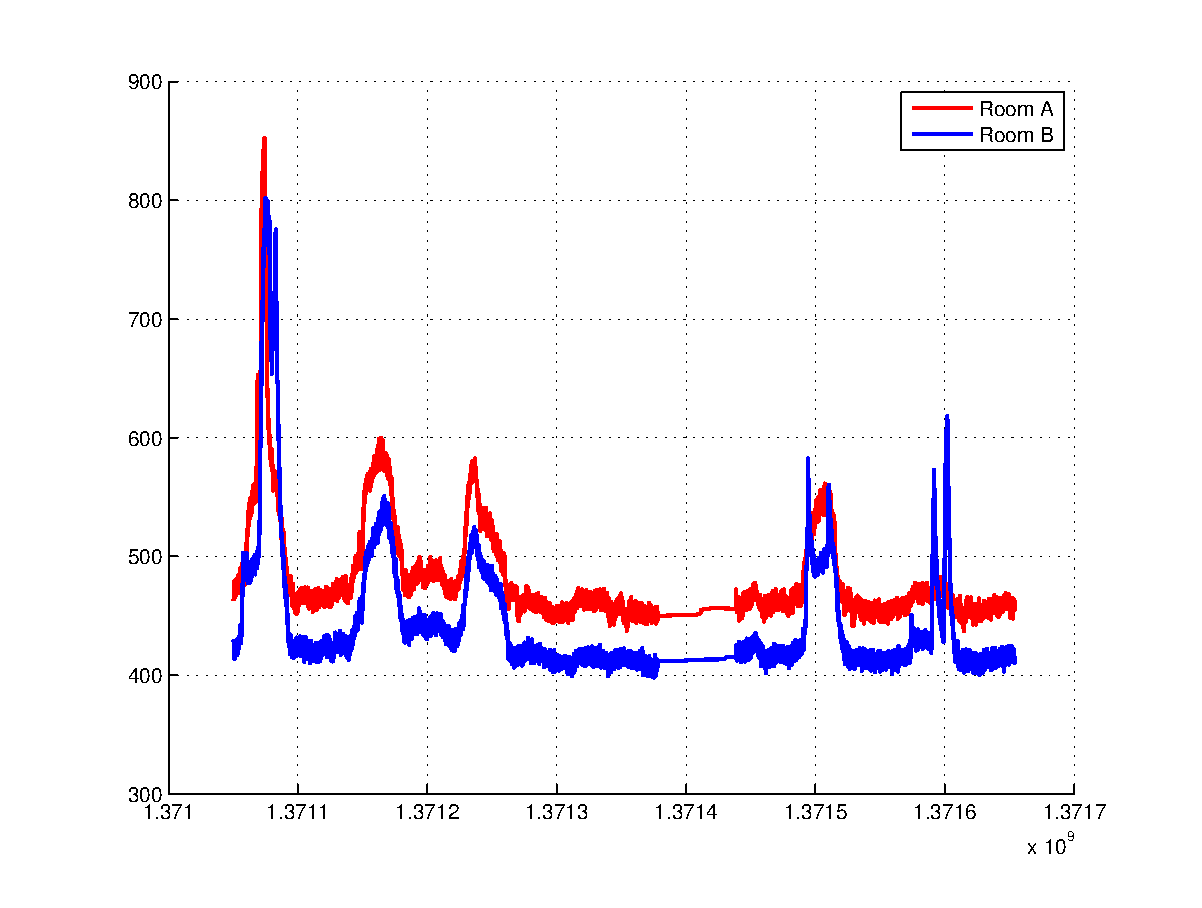
\includegraphics[width=0.48\textwidth]{figs/co2_pair.eps}
%    \caption{CO2 sensor traces.}
%\label{fig:co2traces}
%\end{figure}
%
%\begin{figure}[h!]
%\centering
%    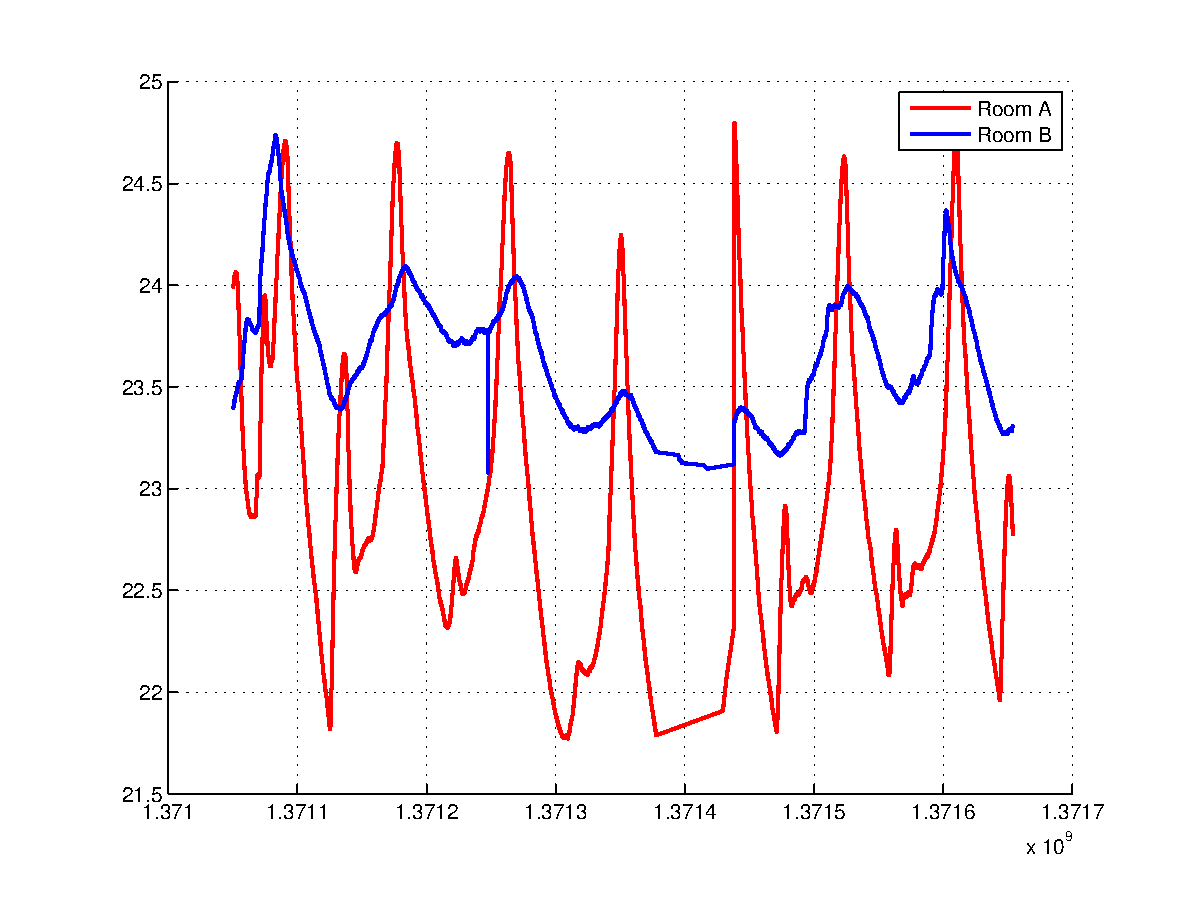
\includegraphics[width=0.48\textwidth]{figs/temp_pair.eps}
%    \caption{temperature traces.}
%\label{fig:temptraces}
%\end{figure}

% tie this into search; search is done for scale
% scale is necessary for broad impact
% 

% discuss how both can be used to generate more metadata that we can use for indexing



\section{Related Work}

\cite{Harris:2011}
\cite{Gulwani:2011}
\cite{Singh:2012}
\cite{Gulwani12spreadsheetdata}



% \balance
\bibliographystyle{abbrv}
\bibliography{sigproc}  % sigproc.bib is the name of the Bibliography in this case
\end{document}
